\documentclass{beamer}
\usepackage{beamerthemeshadow}
\usepackage[french]{babel}
\usepackage[T1]{fontenc}
\usepackage[utf8x]{inputenc}

\begin{document}
\title{Droits du Numérique}  
\author{GAUTHIER Silvère - EL JAOUHARY Abderrahim}
\date{\today} 

\frame{\titlepage} 

\frame{\frametitle{Plan}\tableofcontents}


\section{Introduction}
\subsection{Bref historique}
\frame{\frametitle{Début de l'ère numérique}
L'apparition et le développement du numérique pause de nombreux problèmes législatifs et juridiques.\newline
\bigskip

Il est nécessaire de mettre en place un système de droit adapté au numérique.
}

\subsection{Droit de l'informatique}
\frame{\frametitle{Droit de l'informatique}
\begin{block}{Définition}
	\begin{itemize}
	\item Ensemble des dispositions relatives aux NTIC.
	\end{itemize}
\end{block}
On ne peut toutefois pas le décrire comme une unité organique telle que le droit civil ou le droit commercial.
Il consiste plutôt en \textbf{modifications} d'un grand nombre de domaines existants du droit.
}

\subsection{Droit d'internet}
\frame{\frametitle{Droit d'internet}
\begin{block}{Définition}
	\begin{itemize}
	\item Ensemble des règles de droit \textbf{applicables} à internet.
	\end{itemize}
\end{block}
Le droit d’internet n’est pas une branche du droit autonome. Il s’agit donc d’un droit qui s’applique à internet, mais qui ne lui est pas propre.
}

\subsection{Définitions}
\frame{\frametitle{Quelques définitions...}
\begin{block}{Droit positif}
	\begin{itemize}
	\item Droit consistant à \textbf{autoriser} une action.
	\end{itemize}
\end{block}
\begin{block}{Droit négatif}
	\begin{itemize}
	\item Droit consistant à \textbf{interdire} une action.
	\end{itemize}
\end{block}
\begin{block}{TIC / NTIC}
	\begin{itemize}
	\item Nouvelles technologies de l'information et de la communication (NTIC).
	\end{itemize}
\end{block}
\begin{block}{Neutralité du réseau}
	\begin{itemize}
	\item Principe qui garantit l'égalité de traitement de tous les flux de données sur Internet.
	\end{itemize}
\end{block}
}

\section{Droits, lois et organismes}
\frame{\frametitle{Droits}
\begin{itemize}
\item \textbf{Droit d'auteur :} \footnotesize ensemble des prérogatives exclusives dont dispose un auteur ou ses ayants droit.\normalsize
\pause
\item \textbf{Droits voisins :} \footnotesize partie particulière de la propriété littéraire et artistique en droit français.\normalsize
\pause
\item \textbf{Droit des marques :} \footnotesize monopole d'exploitation de ce signe pour le type de produits ou services qu'il accompagne.\normalsize
\pause
\item \textbf{Brevet :} \footnotesize droit d'interdiction de l'exploitation de l'invention par un tiers.\normalsize
\pause
\item \textbf{Propriété intellectuelle :} \footnotesize ensemble des droits accordés sur les créations intellectuelles à l'auteur ou à l'ayant droit d'une œuvre de l'esprit.\normalsize
\pause
\item \textbf{Droit des télécommunications :} \footnotesize droit relatif à toute transmission, émission ou réception.\normalsize %de signes, de signaux, d’écrits, d’images, de sons ou de renseignements de toute nature, à distance, par fil, radioélectricité, optique ou d’autres système électromagnétiques
\end{itemize}
}
\frame{\frametitle{Devoirs}
\begin{itemize}
\item Respect de la vie privée
\item Obligation d'information %e-commerce, FAI, charte de sites en créant un compte
\end{itemize}
}
\frame{\frametitle{Libertés}
\begin{itemize}
\item Liberté d'expression
\item Respect de la vie privée
\item Respect de la confidentialité de la communication...
\end{itemize}
\bigskip

Ces libertés reposent techniquement sur la Neutralité du réseau.
}
\frame{\frametitle{Lois}
\begin{itemize}
\item DMCA (us, 1998) :  \footnotesize lutte contre les violations du droit d'auteur.\normalsize
\pause
\item DADVSI (fr, 2006) : \footnotesize harmonise droit d'auteur et droits voisins dans la société de l'information.\normalsize
\pause
\item Hadopi 1 (fr, 2009) : \footnotesize vise à stopper le « peer to peer » illégal.\normalsize
\pause
\item Hadopi 2 (fr, 2009) : \footnotesize protection de la propriété littéraire et artistique sur internet.\normalsize
\pause
\item ACTA (inter, 2011) : \footnotesize renforcement des droits de propriété intellectuelle.\normalsize
\end{itemize}
}
\frame{\frametitle{Organismes}
\begin{itemize}
\item CNIL (fr, 1978) : \footnotesize veiller au respect de l'identité, des droits, de la vie privée et des libertés dans le domaine de l'informatique.\normalsize
\pause
\item TCG (inter, 2003) : \footnotesize sécuriser les équipements et communications informatiques.\normalsize
\pause
\item ARMT (fr, 2007) : \footnotesize surveillance des DRM.\normalsize
\pause
\item OMPI (inter, 2008) : \footnotesize promouvoir un système international de propriété intellectuelle.\normalsize
\pause
\item HADOPI (fr, 2009) : \footnotesize protection des intérêts des titulaires de droits d'œuvres protégées.\normalsize
\end{itemize}
}

\section{Gestion des droits}
\subsection{Les DRM}
\frame{\frametitle{Digital Rights Managements}
\begin{itemize}
\item \textbf{But :} réguler l'utilisation des oeuvres numériques.
\item \textbf{Support :} tout type de support numérique physique ou de transmission. 
\item \textbf{Technique :} système d'accès conditionnel (CAS) et chiffrement, licence.
\end{itemize}
}
\frame{\frametitle{Applications}
\begin{itemize}
\item Diffusion TV (satellite, câble, hertzien)
\item Périphériques multimedia
\item Informatique
\end{itemize}
}
\frame{\frametitle{Limites et conséquences}
\textbf{Limites techniques :}\newline
un fichier chiffré reste parfaitement copiable, toute oeuvre numérique finit par être convertie en analogique (trou analogique)...
\bigskip

\textbf{Conséquences :}\newline
copie privée, parodie et citation deviennent impossibles, les DRM deviennent une atteinte à la vie privée...
}

\subsection{Informatique de confiance}
\frame{\frametitle{Principe}
Projet de grandes sociétés d'informatique.\newline
\bigskip

Le principe de base est d'assigner une signature à chaque objet informatique (logiciel, document), et à déléguer à un tiers de confiance la tâche de vérifier si l’objet manipulé est autorisé à être utilisé sur le système informatique local.
}
\frame{\frametitle{Technologies}
\begin{block}{Puce TPM ou Fritz}
Composant cryptographique matériel (passif).
\end{block}
\begin{itemize}
\item NGSCB : ordinateur sécurisé de la prochaine génération.
\item Tatouage numérique.
\end{itemize}
% \begin{block}{Indication géographique}
% 	\begin{itemize}
% 	\item Nom, appellation ou symbole appliqué à certains produits ou services qui correspond à une localisation géographique ou à une origine spécifiques.
% 	\end{itemize}
% \end{block}
}

\section{Discussion}
\subsection{Censure}
\frame{\frametitle{Filtrage d'internet}
\begin{block}{Définition}
Ensemble de techniques visant à limiter l'accès à certains sites normalement accessibles sur le réseau Internet.
\end{block}
Le problème du filtrage est son penchant vers la censure...
}
\frame{\frametitle{"Enemis d'internet"}
Selon Reporters Sans Frontières (RSF), voici les pays jugés \newline
"enemis d'internet" au 12/03/2012\newline
%IMG : Enemis d'internet
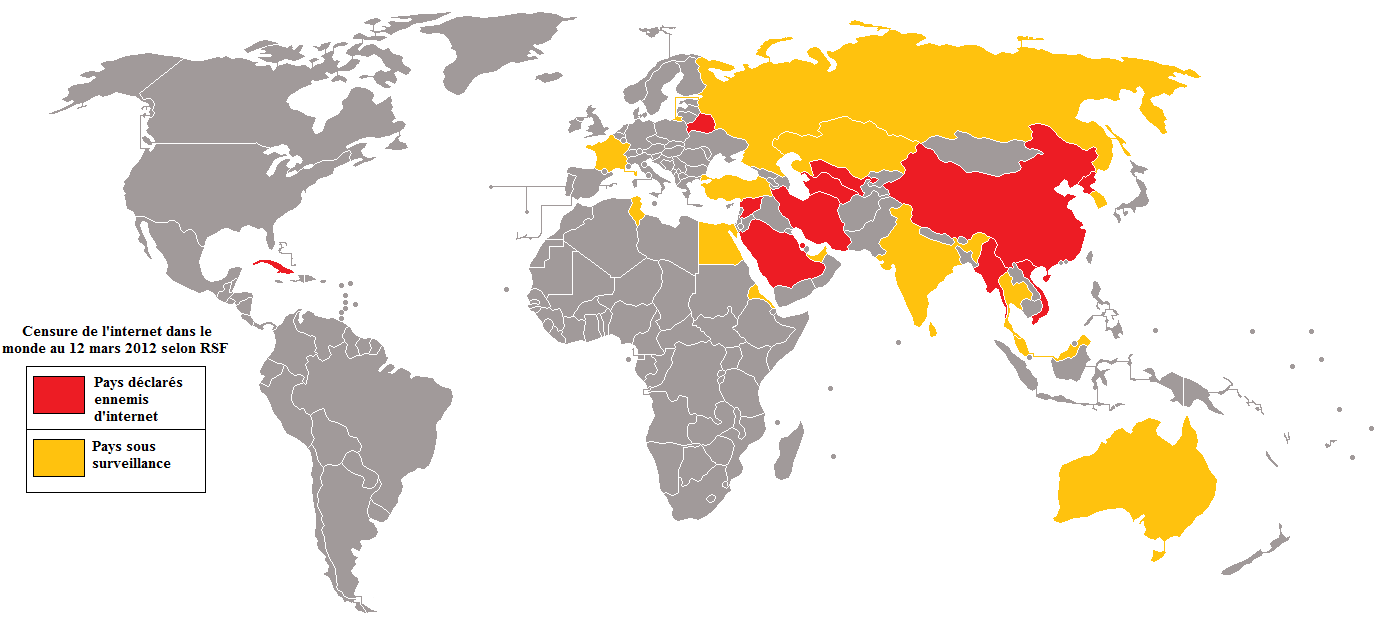
\includegraphics[scale=0.325]{RSF-internet-2012-03-12.png}
}
\frame{\frametitle{Contournements}
Différentes techniques :
\begin{itemize}
\item proxy
\item logiciels
\item sites miroirs...
\end{itemize}
}

\subsection{Anecdotes}
\frame{\frametitle{Quelques anecdotes...}
\begin{itemize}
\item Invention du magnétoscope
\pause
\item Big Brother Awards
\pause
\item Les Anonymous
\pause
\item Affaire Pirate Bay
\end{itemize}
}

\section{Conclusion}
\frame{\frametitle{Notre liberté s'arrête là où celle des autres commence...}
Une loi, la LPD (ch, 1992), est censée réguler la cryptographie : 
\begin{itemize}
\item Données sensibles
\item Limites
\end{itemize}
}
\frame{\frametitle{Conclusion}
Beaucoup de contradictions entre besoins, lois et libertés...\newline
Notions de droit du numérique parfois ambigüe.
\bigskip

Tout comme le reste du droit...
}

\section{Sources}
\frame{\frametitle{Sources}
Sites internets :
\footnotesize 
	\begin{itemize}
	\item fr.wikipedia.org%/wiki/
	\item www.cnil.fr
	\item www.foruminternet.org/specialistes/veille-juridique/textes-officiels/
	\item webdroits.fr
	\item www.numerama.com%/magazine/4373-the-pirate-bay-l-enquete-confirme-les-pressions-americaines.html
	\item www.vieprivee.com
	\item www.bigbrotherawards.org
	%\item bigbrotherawards.eu.org
	\item en.rsf.org
	\item www.admin.ch%/ch/f/rs/235\_1/index.html
	\item www.hadopi.fr%/la-haute-autorite/la-commission-de-protection-des-droits-presentation-et-missions
	\item www.sos-hadopi.fr
	\end{itemize}
\normalsize
}
\frame{\frametitle{Sources (suite)}
Vidéos et Animations :
\footnotesize 
	\begin{itemize}
	\item www.dvanw.com/misopoint/drm/index.html
	\item vimeo.com/28381159
	\item www.youtube.com%/watch?v=RatR_GVtVqo
	\end{itemize}
\normalsize
\bigskip

Livres : 
\footnotesize 
	\begin{itemize}
	\item Internet et le droit, Olivier Iteanu, \textit{éditions Eyrolles}, avril 1996
	\end{itemize}
\normalsize
}
\end{document}

